\documentclass[11pt,a4paper]{article}

%% ── packages ──────────────────────────────────────────────────────
\usepackage[utf8]{inputenc}
\usepackage[T5,T1]{fontenc}
\usepackage[vietnamese]{babel}
\usepackage{microtype}
\usepackage{geometry}
\geometry{margin=2.4cm}
\usepackage{booktabs,array}
\usepackage{graphicx}
\usepackage{xcolor}
\usepackage{hyperref}
\usepackage{enumitem}
\usepackage{caption}
\usepackage{subcaption}
\usepackage{amsmath,amssymb}
\usepackage{setspace}
\usepackage{parskip}
\usepackage{tikz}
\usetikzlibrary{arrows.meta,positioning,shapes.geometric,fit,backgrounds,calc}
\usepackage[numbers,sort&compress]{natbib}

%% ── diagram palette & node styles ─────────────────────────────────
\definecolor{cData}{HTML}{2C6E9B}   % data / raw sources
\definecolor{cProc}{HTML}{3F8A5B}   % processing / features
\definecolor{cBase}{HTML}{B0642A}   % intensity-only baselines
\definecolor{cCov}{HTML}{7A3E9D}    % covariate-using models (this work)
\definecolor{cEval}{HTML}{555555}   % evaluation
\definecolor{cPass}{HTML}{2E8B57}   % gate: pass
\definecolor{cFail}{HTML}{B03A2E}   % gate: reject

\tikzset{
  box/.style={rounded corners=2pt, draw=#1, line width=0.9pt, fill=#1!8,
              text=black, align=center, font=\small, inner sep=5pt,
              minimum height=8mm},
  data/.style={box=cData},
  proc/.style={box=cProc},
  base/.style={box=cBase},
  cov/.style={box=cCov},
  eval/.style={box=cEval},
  gate/.style={diamond, aspect=2, draw=cEval, line width=0.9pt, fill=cEval!8,
               align=center, font=\small, inner sep=2pt},
  flow/.style={-{Stealth[length=2.4mm]}, line width=0.8pt, draw=cEval},
  flowd/.style={flow, dashed},
  lbl/.style={font=\scriptsize\itshape, text=cEval},
}

%% ── metadata ──────────────────────────────────────────────────────
\title{\textbf{Phân tích Khám phá Dữ liệu \& Kết quả Ban đầu}\\%
       \large Yếu tố Đông đúc theo Tầng Ví (Tier-Aware Crowding) và\\
       Cảnh báo sớm các Đợt Bùng phát Thanh lý Đồng bộ\\
       trên Thị trường Hợp đồng Tương lai Vĩnh cửu On-chain}
\author{Luận văn Thạc sĩ Khoa học Máy tính}
\date{Tháng 7, 2026}

\begin{document}
\maketitle

\begin{abstract}
Báo cáo này phát triển và kiểm chứng độ khả thi cho một hướng nghiên cứu luận văn mới, dựa trên cơ sở dữ liệu \texttt{perpetuals\_knowledge\_graph} (40,5 triệu sự kiện log, 1,34 triệu vị thế đã đóng, 190\,573 sự kiện thanh lý tường minh, 249 tài sản, 5 sàn giao dịch, 491 ngày dữ liệu). Chúng tôi dự báo các \emph{đợt bùng phát thanh lý đồng bộ} (synchronized liquidation bursts)---những khoảng thời gian ngắn trong đó nhiều vị thế hợp đồng tương lai vĩnh cửu (perpetual futures) trên cùng một tài sản bị đóng cưỡng bức cùng lúc---và đặt câu hỏi liệu các đặc trưng \emph{đông đúc theo tầng ví} (tier-aware crowding) có cải thiện khả năng dự báo so với mô hình nền tự kích thích (self-exciting) kiểu Hawkes hay không. Hai thử nghiệm khả thi được thực hiện trước khi xây dựng bất kỳ mô hình nào. (i) Giả thuyết \emph{"nam châm thanh lý"} (giá bị hút về các vùng giá thanh lý dày đặc) đã bị \textbf{bác bỏ} trên ba tài sản thanh khoản cao nhất, dưới hai dạng kiểm định độc lập (đều cho kết quả null). (ii) Nhãn \emph{bùng phát thanh lý} (burst) đã \textbf{vượt qua thử nghiệm một cách thuyết phục}: nhãn này dày đặc và có khả năng học mạnh---chỉ một đặc trưng cường độ trễ (trailing-intensity) đơn lẻ đã đạt AUC $0{,}83$--$0{,}87$, xác nhận hiện tượng tự kích thích. Trên một phép chia dữ liệu theo thời gian, an toàn không rò rỉ (4,2 triệu dòng tài sản-khung giờ, 40 tài sản), một mô hình gradient boosting được tinh chỉnh với đặc trưng đông đúc (mất cân bằng theo tầng, lan tỏa liên tài sản, giá trị danh nghĩa thanh lý; 17 đặc trưng) được so sánh với ba mô hình nền \emph{có tên gọi, đã công bố}, cùng huấn luyện trên dữ liệu giống nhau: một quá trình Hawkes đơn biến cổ điển (ước lượng hợp lý cực đại), một Hawkes đa biến có thành phần thị trường, và một Transformer Hawkes Process thần kinh (Zuo et al., 2020). Sau đó, ba mô hình sử dụng đặc trưng hiệp biến (covariate) được đánh giá: bộ phân loại đã tinh chỉnh, một quá trình điểm thần kinh (neural point process) có điều kiện hiệp biến (mô hình hazard dựa trên GRU trên chuỗi đặc trưng), và một mạng nơ-ron đồ thị không gian--thời gian (spatio-temporal GNN) trên đồ thị liên tài sản. Trên độ đo precision-recall---thước đo trung thực cho một tập kiểm tra có tỷ lệ dương chỉ $0{,}56\%$---cả ba mô hình đều vượt trội hơn cả ba mô hình nền với khoảng cách lớn; quá trình điểm có điều kiện hiệp biến (CovTPP) đạt kết quả tốt nhất (PR-AUC $0{,}256$, so với $0{,}157$ của Hawkes cổ điển và $0{,}129$ của THP thần kinh, mức tăng từ $+0{,}10$ đến $+0{,}13$), nhỉnh hơn một chút so với GNN ($0{,}251$) và bộ phân loại đã tinh chỉnh ($0{,}250$). Yếu tố quyết định chính là các đặc trưng hiệp biến, được chứng minh \emph{trong cùng một họ mô hình}: quá trình điểm thần kinh gần như \emph{tăng gấp đôi} PR-AUC ($0{,}129\to0{,}256$) khi được điều kiện hóa theo đặc trưng đông đúc thay vì chỉ dựa vào thời điểm sự kiện. Đáng chú ý, tất cả các mô hình nền chỉ dựa trên cường độ (intensity-only) đều đạt ROC-AUC $\approx 0{,}97$ nhưng PR-AUC chỉ $\approx 0{,}13$--$0{,}16$: cường độ tự kích thích là một bộ xếp hạng (ranker) mạnh nhưng là tín hiệu độ chính xác (precision) yếu dưới điều kiện mất cân bằng---điều mà ROC che giấu còn PR-AUC phơi bày. Khác với công thức chấm điểm kỹ năng ví (wallet-scoring) trước đây---nơi nhãn đánh giá gần như $99\%$ là nhiễu lấy mẫu---bài toán này có một nhãn dày đặc, đáng tin cậy, nên mức cải thiện đo được là có ý nghĩa thực chất.
\end{abstract}

%% ===================================================================
\section{Bối cảnh Thể chế (Institutional Background)}
\label{sec:institutional}
%% ===================================================================

Phần này giải thích các khái niệm thị trường được dùng xuyên suốt báo cáo, để người đọc không chuyên về thị trường phái sinh crypto vẫn theo dõi được các phần sau.

\subsection{Hợp đồng tương lai vĩnh cửu (Perpetual Futures) là gì}

Hợp đồng tương lai vĩnh cửu (perpetual futures, viết tắt \emph{perp}) là một công cụ phái sinh cho phép giao dịch có đòn bẩy trên giá của một tài sản (ví dụ BTC, SOL) mà \textbf{không có ngày đáo hạn}---khác với hợp đồng tương lai truyền thống. Vì không có ngày đáo hạn để giá hợp đồng tự động hội tụ về giá giao ngay (spot), cơ chế giữ cho giá perp bám sát giá spot là \textbf{tỷ lệ tài trợ} (funding rate): định kỳ (thường mỗi 1--8 giờ), bên nắm giữ vị thế mua (long) và bên nắm giữ vị thế bán (short) thanh toán một khoản phí nhỏ cho nhau, tỷ lệ thuận với chênh lệch giữa giá perp và giá chỉ số (index/oracle price). Khi giá perp cao hơn giá spot, long trả phí cho short (khuyến khích bán, kéo giá xuống); khi thấp hơn, chiều ngược lại. Perp hiện là công cụ phái sinh crypto phổ biến nhất và ngày càng đóng vai trò trung tâm trong việc khám phá giá (price discovery).

\subsection{Đòn bẩy, Ký quỹ và Cơ chế Thanh lý (Liquidation)}

Một vị thế perp được mở bằng một khoản \textbf{ký quỹ ban đầu} (initial margin) $m$, nhân với \textbf{đòn bẩy} (leverage) $\ell$ để có quy mô vị thế danh nghĩa $s = m \times \ell$ (ví dụ: ký quỹ 100 USD, đòn bẩy 10x $\Rightarrow$ vị thế trị giá 1000 USD). Sàn/giao thức yêu cầu vị thế luôn duy trì một mức \textbf{ký quỹ duy trì} (maintenance margin) tối thiểu, tính theo tỷ lệ ký quỹ hiện tại trên quy mô vị thế. Khi giá thị trường di chuyển ngược hướng vị thế đủ để tỷ lệ ký quỹ giảm xuống dưới ngưỡng duy trì, vị thế đó chạm \textbf{giá thanh lý} (liquidation price)---xấp xỉ
\[
  P_{\text{liq}} \approx P_{\text{entry}} \times \left(1 \mp \frac{1}{\ell}\right) \quad (\text{Long: } -,\ \text{Short: } +),
\]
và bị \textbf{đóng cưỡng bức} (force-closed): sàn/giao thức (hoặc một \emph{keeper}/liquidator bên thứ ba được thưởng phí) tự động đóng vị thế bằng cách khớp một lệnh ngược chiều ra thị trường, bất kể chủ vị thế có đồng ý hay không. Đòn bẩy càng cao, khoảng cách tới giá thanh lý càng hẹp---đây chính là biến định lượng cốt lõi của các đặc trưng "đông đúc" (crowding) trong báo cáo (mức đòn bẩy trung bình, mức tập trung vị thế theo tầng ví).

\subsection{Cơ chế gây ra Đợt Bùng phát Thanh lý (Liquidation Cascade)}

Rủi ro hệ thống đặc trưng của perp là \textbf{thác thanh lý} (liquidation cascade): việc đóng cưỡng bức một vị thế long tạo ra một lệnh \emph{bán} ra thị trường; việc đóng một vị thế short tạo ra một lệnh \emph{mua}. Nếu nhiều vị thế cùng chiều tập trung quanh một vùng giá thanh lý gần nhau (positioning "đông đúc" và một chiều), việc thanh lý loạt vị thế đầu tiên đẩy giá đi xa hơn theo đúng hướng đã gây thanh lý, kích hoạt lớp vị thế đòn bẩy tiếp theo chạm ngưỡng thanh lý của chính nó---một chuỗi phản ứng \textbf{tự kích thích, lây lan} (self-exciting, contagious). Đây chính là cơ chế mà quá trình Hawkes (Eq.~\eqref{eq:intensity}, số hạng thứ hai) mô hình hóa: mỗi sự kiện thanh lý làm tăng tạm thời xác suất xảy ra sự kiện thanh lý tiếp theo. Câu hỏi trung tâm của luận văn là liệu \emph{trạng thái đông đúc hiện tại của thị trường} (crowding state, số hạng $\mu_k(x_k(t))$ trong Eq.~\eqref{eq:intensity})---chứ không chỉ lịch sử sự kiện gần đây---có mang thông tin dự báo được đợt bùng phát \emph{tương lai} hay không.

\subsection{Hai kiến trúc perp on-chain: Hyperliquid và Jupiter}

Dữ liệu của luận văn trải trên 5 sàn/giao thức, nhưng hai kiến trúc đối lập đáng chú ý nhất---và là nguồn dữ liệu giá chính (\texttt{hyperliquid\_prices})---là:

\begin{itemize}[nosep]
    \item \textbf{Hyperliquid}: một sàn perp phi tập trung vận hành trên một blockchain Lớp-1 (L1) riêng do chính Hyperliquid xây dựng, sử dụng cơ chế đồng thuận HyperBFT với thời gian tạo khối dưới một giây. Khớp lệnh theo mô hình \textbf{sổ lệnh giới hạn trung tâm on-chain} (on-chain central limit order book, CLOB)---tương tự sàn tập trung (CEX) truyền thống nhưng toàn bộ sổ lệnh và khớp lệnh đều diễn ra on-chain. Một \emph{vault} nội bộ (HLP) đóng vai trò nhà tạo lập thị trường và hấp thụ một phần rủi ro thanh lý khi thanh khoản sổ lệnh không đủ.
    \item \textbf{Jupiter Perpetuals} (trên Solana): không dùng sổ lệnh, mà dùng mô hình \textbf{giao dịch đối ứng với hồ thanh khoản} (pool-based/peer-to-pool): mọi trader giao dịch trực tiếp với một hồ thanh khoản chung (JLP pool), hồ này đóng vai trò đối tác cho mọi vị thế và gánh lãi/lỗ ròng của toàn bộ trader. Giá tham chiếu để định giá vị thế và xác định thời điểm thanh lý lấy từ \textbf{oracle} giá bên ngoài (ví dụ Pyth Network) thay vì từ khớp lệnh nội bộ.
\end{itemize}

Sự khác biệt kiến trúc này (sổ lệnh vs.\ hồ thanh khoản, cơ chế giá nội sinh vs.\ oracle) là lý do báo cáo không giả định một cơ chế thanh lý thống nhất duy nhất, mà xây dựng nhãn bùng phát Eq.~\eqref{eq:burst} và các đặc trưng đông đúc \S\ref{sec:formulation} một cách \emph{bất khả tri với sàn} (venue-agnostic), gộp sự kiện thanh lý từ \texttt{close\_action = Liquidate} trên toàn bộ 5 sàn/chuỗi, đồng thời giữ venue như một \emph{mark} tùy chọn trong công thức cường độ đa biến (Eq.~\eqref{eq:intensity}).

\subsection{Đầu ra của mô hình: hệ thống dự đoán điều gì}

Với mỗi tài sản $a$ và mỗi khung 5 phút $t$, hệ thống dự đoán một \textbf{xác suất nhị phân}: liệu trong cửa sổ $h$ phút tiếp theo, số lượng sự kiện thanh lý trên tài sản $a$ có đạt hoặc vượt ngưỡng $\theta$ hay không (định nghĩa hình thức tại Eq.~\eqref{eq:burst}, \S\ref{sec:formulation}). Đây \textbf{không phải} là dự đoán chiều giá (tăng/giảm), cũng không phải dự đoán một sự kiện thanh lý đơn lẻ, mà là dự đoán \emph{cụm sự kiện đồng bộ}---một tín hiệu cảnh báo sớm rủi ro thác thanh lý, hướng tới ứng dụng thực tế: cảnh báo cho nhà quản lý rủi ro hoặc chính trader trước khi một đợt bùng phát xảy ra.

%% ===================================================================
\section{Phát biểu Bài toán}
\label{sec:formulation}
%% ===================================================================

\subsection{Vì sao Dự báo Đợt Bùng phát Thanh lý}

Hợp đồng tương lai vĩnh cửu là công cụ phái sinh crypto phổ biến nhất và ngày càng là nơi khám phá giá chính. Rủi ro hệ thống đặc trưng của chúng là \emph{thác thanh lý}: khi một cụm vị thế đòn bẩy vi phạm ngưỡng ký quỹ duy trì, các lệnh thanh lý cưỡng bức bán ra thị trường, đẩy giá đi xa hơn, và kích hoạt lớp vị thế đòn bẩy tiếp theo---một chuỗi tháo chạy tự kích thích, lây lan. Các tín hiệu cảnh báo sớm hiện có mà giới thực hành sử dụng (tỷ lệ tài trợ cực đoan, mất cân bằng long/short, open interest kỷ lục) là các ngưỡng heuristic, không phải mô hình dự báo đã hiệu chỉnh. Luận văn này đặt một câu hỏi sắc bén hơn, có thể học được: \emph{cho trạng thái thị trường tại thời điểm $t$, xác suất xảy ra một đợt bùng phát thanh lý đồng bộ trong $h$ phút tiếp theo là bao nhiêu, và các đặc trưng đông đúc phân giải theo tầng ví có cải thiện dự báo đó so với một mô hình nền thuần túy tự kích thích hay không?}

\subsection{Định nghĩa Hình thức của Đợt Bùng phát}

Gọi $L_{a,t}$ là số sự kiện thanh lý của tài sản $a$ trong khung 5 phút $t$ (nguồn: \texttt{close\_action = Liquidate}). Nhãn bùng phát tại tầm dự báo $h$ (tính theo số khung) và ngưỡng $\theta$ là
\begin{equation}
Y^{(h)}_{a,t} \;=\; \mathbf{1}\!\left[\ \sum_{\tau \in (t,\,t+h]} L_{a,\tau}\ \ge\ \theta\ \right].
\label{eq:burst}
\end{equation}
Nhãn chỉ sử dụng cửa sổ \emph{tương lai} $(t, t+h]$; mọi biến dự báo được tính trên cửa sổ \emph{quá khứ} $[t-w, t]$, do đó đặc trưng và nhãn tách biệt nhau theo cấu trúc. Mục~\ref{sec:m0burst} cố định điểm vận hành tại $h=3$ khung ($15$ phút), $\theta=3$.

\subsection{Phân rã Cường độ Bùng phát}

Chúng tôi mô hình hóa cường độ điều kiện của các sự kiện thanh lý cho tài sản $a$ (và, trong mô hình đầy đủ, các \emph{mark} tầng ví và sàn giao dịch $k$) như một quá trình tự kích thích với một hàm nền điều kiện hóa theo hiệp biến:
\begin{equation}
\lambda_k(t) \;=\; \underbrace{\mu_k\!\big(x_k(t)\big)}_{\text{hàm nền điều kiện hóa theo đông đúc}} \;+\; \sum_{k'}\sum_{t_j < t} \alpha_{k'\to k}\,\phi(t - t_j),
\label{eq:intensity}
\end{equation}
trong đó $\phi$ là hạt nhân kích hoạt dạng mũ (exponential triggering kernel), $\alpha_{k'\to k}$ là ma trận kích thích chéo-mark (lây lan chéo-tầng, chéo-sàn), và $x_k(t)$ là véc-tơ các hiệp biến \emph{đông đúc theo tầng ví}. Số hạng thứ hai là tự kích thích Hawkes cổ điển của \citet{bacry2015hawkes}; thành phần mới là hàm nền điều kiện hóa theo đông đúc $\mu_k(\cdot)$. Giả thuyết trung tâm của luận văn là $x_k(t)$ mang thông tin về các đợt bùng phát \emph{tương lai} vượt ra ngoài những gì lịch sử sự kiện gần đây có thể cung cấp. Hình~\ref{fig:intensity} ánh xạ mỗi họ mô hình vào hai số hạng của Eq.~\eqref{eq:intensity}.

%% ── Fig: intensity decomposition ─────────────────────────────────
\begin{figure}[ht]
\centering
\begin{tikzpicture}[node distance=6mm and 10mm]
  \node[cov] (mu) {\textbf{Hàm nền đông đúc} $\mu_k(x_k(t))$\\\scriptsize mất cân bằng theo tầng, tập trung,\\\scriptsize đòn bẩy, lan tỏa liên tài sản};
  \node[base, right=24mm of mu] (self) {\textbf{Tự kích thích}\\$\sum_{k'}\sum_{t_j<t}\alpha_{k'\to k}\,\phi(t-t_j)$\\\scriptsize hạt nhân mũ trên sự kiện quá khứ};
  \node[eval, below=12mm of $(mu)!0.5!(self)$] (lam) {$\lambda_k(t)$\\\scriptsize cường độ bùng phát điều kiện};

  \draw[flow, draw=cCov] (mu) -- (lam);
  \draw[flow, draw=cBase] (self) -- (lam);

  % which model touches which term
  \node[lbl, below=1mm of self, text=cBase] {Hawkes / THP chỉ nắm bắt số hạng \emph{này}};
  \node[lbl, below=1mm of mu, text=cCov] {CovTPP / ST-GNN / LGBM bổ sung số hạng \emph{này}};
\end{tikzpicture}
\caption{Phân rã cường độ bùng phát, Eq.~\eqref{eq:intensity}. Các mô hình nền đã công bố chỉ mô hình hóa số hạng tự kích thích (phải); các mô hình sử dụng hiệp biến trong luận văn này cung cấp hàm nền điều kiện hóa theo đông đúc (trái). Luận văn đo \emph{mức tăng} khi bổ sung số hạng bên trái, được tách bạch rõ nhất trong họ TPP thần kinh (THP $\to$ CovTPP).}
\label{fig:intensity}
\end{figure}

\subsection{Giả thuyết Đông đúc (Crowding Hypothesis)}

Đông đúc làm mỏng "biên độ an toàn" của thị trường: khi vị thế tập trung và lệch một chiều---đặc biệt ở các ví lớn---một biến động bất lợi vừa phải cũng đủ thanh lý nhiều vị thế cùng lúc. Do đó, với mỗi tài sản và mỗi khung 5 phút, chúng tôi xây dựng các đặc trưng mà một đại lượng vô hướng đơn lẻ như tỷ lệ tài trợ không thể biểu đạt được: mất cân bằng long/short theo open interest, mất cân bằng theo từng tầng (ví nhỏ/trung/lớn), độ bất đồng nhỏ-so-với-lớn, mức độ tập trung vị thế, đòn bẩy trung bình của các vị thế đang mở, và tốc độ biến thiên của các đại lượng này. Mục tiêu dự đoán Eq.~\eqref{eq:burst} kiểm định trực tiếp liệu các hiệp biến này có làm tăng xác suất bùng phát hay không.

\subsection{Bài toán Đánh giá (và Tương phản với Wallet Skill)}

Một công thức trước đây trên cùng cơ sở dữ liệu---chấm điểm kỹ năng ví theo chiều giao dịch (side-aware wallet skill scoring)---thất bại vì lý do đo lường: nhãn đánh giá của nó (tỷ lệ thắng tương lai trên một số ít giao dịch) gần như $99\%$ là nhiễu lấy mẫu nhị thức, nên không phương pháp nào có thể chứng minh vượt trội hơn các mô hình nền đơn giản. Công thức hiện tại được lựa chọn có chủ đích để tránh cái bẫy đó. Nhãn bùng phát Eq.~\eqref{eq:burst} là một \emph{đếm sự kiện} trên một luồng dữ liệu dày đặc (190\,573 lượt thanh lý), không phải một tỷ lệ nhiễu theo từng ví. Mục~\ref{sec:m0burst} cho thấy nhãn này có khả năng học mạnh. Hệ quả là mục tiêu mô hình hóa không còn là "liệu bùng phát có dự đoán được không" (câu trả lời gần như hiển nhiên là có, nhờ tự tương quan thời gian) mà là \emph{đặc trưng đông đúc cải thiện dự báo thêm bao nhiêu so với mô hình nền tự kích thích}---một câu hỏi được đặt ra rõ ràng, đo lường được.

\subsection{Đóng góp}

Tóm gọn trong một câu: \emph{hiệp biến đông đúc, khi được tiêm vào hàm nền cường độ của một quá trình tự kích thích, gần như tăng gấp đôi PR-AUC so với các mô hình nền quá trình điểm chỉ dựa vào cường độ, trên một dự báo bùng phát thanh lý ngoài mẫu, an toàn không rò rỉ.} Cụ thể:

\begin{itemize}[nosep]
    \item \textbf{(C1)} Một bảng đông đúc phân giải theo tầng ví và nhãn bùng phát an toàn không rò rỉ, xây dựng từ 40,5 triệu sự kiện on-chain thô (4,24 triệu dòng tài sản-khung, 40 tài sản; \S\ref{sec:system}--\S\ref{sec:m0burst}), với hai thử nghiệm khả thi được chạy \emph{trước khi} mô hình hóa để giảm rủi ro hướng đi.
    \item \textbf{(C2)} Một quá trình điểm thần kinh điều kiện hóa theo hiệp biến (CovTPP) hiện thực hóa hàm nền điều kiện hóa theo đông đúc $\mu_k(\cdot)$ của Eq.~\eqref{eq:intensity}, tách bạch hiệu ứng hiệp biến \emph{trong cùng} họ TPP thần kinh, đối chứng với mô hình nền Transformer Hawkes Process.
    \item \textbf{(C3)} Các đặc trưng lan tỏa liên tài sản tường minh và một GNN không gian--thời gian trên đồ thị vị thế, đối chứng với một quá trình Hawkes đa biến có thành phần thị trường.
    \item \textbf{(C4)} Một đánh giá ưu tiên precision-recall trên các khung kiểm tra ngoài mẫu giống hệt nhau, qua sáu mô hình có tên gọi (\S\ref{sec:results}), phơi bày một sự phân kỳ ROC/PR mà báo cáo chỉ dựa vào ROC sẽ che giấu.
\end{itemize}

\S\ref{sec:gap} định vị mỗi đóng góp đối chứng với một khoảng trống cụ thể, có trích dẫn, trong các công trình trước đây.

%% ===================================================================
\section{Công trình Liên quan (Related Work)}
\label{sec:related}
%% ===================================================================

Chúng tôi tổ chức các công trình liên quan theo năm hướng nghiên cứu mà luận văn này nằm ở giao điểm, và nêu rõ tại \S\ref{sec:gap} chính xác vị trí mỗi hướng còn thiếu so với một dự báo bùng phát thanh lý có hiệu chỉnh, nhận biết đông đúc.

\paragraph{Quá trình tự kích thích và thác thanh lý.} Mô hình hóa các sự kiện tài chính tập trung thành cụm như quá trình tự kích thích (Hawkes) đã được thiết lập vững chắc: \citet{bacry2015hawkes} khảo sát quá trình Hawkes trong tài chính, và \citet{hardiman2013endogeneity} dùng tỷ lệ phân nhánh (branching ratio) để định lượng tính nội sinh/phản xạ của thị trường (endogeneity/reflexivity)---cùng cơ chế mà \citet{filimonov2012reflexivity} gắn với các đợt sụp đổ chớp nhoáng (flash crash). Công trình DeFi gần nhất, \citet{cao2025defi}, cho thấy các sự kiện thanh lý tập trung thành cụm \emph{xuyên} nhiều giao thức trong một khung Hawkes đa biến, còn \citet{markovhawkes2025manipulation} mở rộng cường độ Hawkes với một hàm nền điều biến kiểu Markov để phát hiện thao túng thị trường. Toàn bộ hướng này mô hình hóa cường độ chỉ từ \emph{lịch sử sự kiện} (Eq.~\eqref{eq:intensity}, số hạng thứ hai); trạng thái vị thế/đông đúc không bao giờ đi vào hàm nền $\mu_k$. Một hướng nowcasting song song \citep{nowcast2023crashrisk} dự đoán rủi ro sụp đổ từ mất cân bằng dòng lệnh (order-flow imbalance) nhưng không dựa trên vị thế phân giải theo tầng ví.

\paragraph{Vi cấu trúc thị trường perpetual và rủi ro thanh khoản.} Rủi ro thanh khoản hướng tới tương lai cho perp bắt đầu thu hút các khung phân tích chuyên biệt như Slippage-at-Risk \citep{slippageatrisk2026}, định lượng rủi ro thực thi lệnh nhưng coi thanh lý là một cú sốc thanh khoản ngoại sinh, chứ không phải một luồng sự kiện tự kích thích, dự báo được.

\paragraph{Quá trình điểm thời gian có mark và thần kinh (neural TPP).} Một họ mô hình phong phú điều kiện hóa cường độ sự kiện theo lịch sử đã học: quá trình điểm thời gian có mark hồi quy \citep{du2016rmtpp}, quá trình Hawkes thần kinh \citep{mei2017neuralhawkes}, Transformer Hawkes Process \citep{zuo2020thp}, quá trình điểm thần kinh không gian--thời gian \citep{zhou2022neuralstpp}, dự báo đa sự kiện không gian--thời gian \citep{beyondhawkes2022}, và các biến thể state-space gần đây \citep{mambahawkes2024}, nay được đối chứng công khai bởi EasyTPP \citep{xue2023easytpp}. Các phương pháp này điều kiện hóa theo thời điểm sự kiện và \emph{mark} phân loại, nhưng---như mô hình nền THP của chúng tôi cho thấy bằng thực nghiệm---không điều kiện hóa theo các hiệp biến đông đúc liên tục, ngoại sinh; bộ máy thần kinh nâng cao độ biểu đạt so với Hawkes cổ điển nhưng vẫn rơi vào cùng dải độ chính xác khi chỉ được cấp thời điểm sự kiện (Bảng~\ref{tab:m2}).

\paragraph{Cấu trúc tô-pô và liên tài sản của đồ thị on-chain.} Cấu trúc mạng blockchain mang tín hiệu cảnh báo sớm: phát hiện bất thường tô-pô trên mạng đa lớp động \citep{oforiboateng2021topological}, đặc trưng tô-pô cho dự đoán bất thường giá \citep{xrp2026topological}, và phát hiện bất thường mạng theo tốc độ bền vững (persistence velocity) \citep{persistencevelocity2025}. Những công trình này là động lực cho đồ thị liên tài sản của chúng tôi (ST-GNN, \S\ref{sec:results}) nhưng nhắm tới bất thường giá/nhãn trên đồ thị giao dịch, không phải các đợt bùng phát thanh lý đồng bộ trên một đồ thị vị thế liên tài sản.

\paragraph{Dự đoán conformal dưới dịch chuyển phân phối.} Vì tần suất bùng phát bị dịch chuyển (tỷ lệ nền tập kiểm tra $0{,}56\%$ so với tập huấn luyện $1{,}51\%$, \S\ref{sec:results}), độ bất định đã hiệu chỉnh phải sống sót qua tính phi dừng: suy luận conformal thích nghi \citep{gibbs2021adaptive}, dự đoán conformal cho chuỗi thời gian \citep{zaffran2022adaptive}, và luồng conformal nhận biết dịch chuyển \citep{driftconformal2026}. Các công trình này cung cấp tầng hiệu chỉnh cho hệ thống được hoạch định nhưng chưa từng được áp dụng cho một quá trình điểm bùng phát thanh lý.

%% ===================================================================
\section{Khoảng trống Nghiên cứu và Đóng góp}
\label{sec:gap}
%% ===================================================================

Đọc năm hướng nghiên cứu cùng nhau, ta thấy một giao điểm cụ thể còn bỏ trống.

\begin{enumerate}[label=\textbf{G\arabic*:},leftmargin=*]
    \item \textbf{Mô hình thác thanh lý chỉ dựa vào cường độ bỏ qua đông đúc.} Các mô hình thanh lý DeFi/tài chính \citep{cao2025defi,bacry2015hawkes,hardiman2013endogeneity} dự báo chỉ từ lịch sử sự kiện. Liệu vị thế \emph{phân giải theo tầng ví} (mất cân bằng, tập trung, đòn bẩy) có bổ sung sức mạnh dự báo so với tự kích thích hay không---vẫn chưa được kiểm định.
    \item \textbf{TPP thần kinh chưa được điều kiện hóa theo đông đúc ngoại sinh.} Các quá trình điểm hiện đại nhất \citep{zuo2020thp,mei2017neuralhawkes,du2016rmtpp} điều kiện hóa theo thời điểm và mark, không theo một luồng hiệp biến liên tục về vị thế thị trường---nên câu hỏi hiệp biến-đối-cường độ chưa được tách bạch \emph{trong cùng một họ mô hình}.
    \item \textbf{Lây lan xuyên giao thức mới chỉ được mô tả, chưa được dự báo.} \citet{cao2025defi} thiết lập cụm lây lan xuyên giao thức theo hướng mô tả; chưa công trình nào biến lan tỏa liên tài sản thành một dự báo \emph{cảnh báo sớm} có hiệu chỉnh, an toàn không rò rỉ, cho đợt bùng phát tiếp theo.
    \item \textbf{Chưa có cảnh báo sớm bùng phát đã hiệu chỉnh, nhận biết dịch chuyển.} Các phương pháp conformal \citep{gibbs2021adaptive,zaffran2022adaptive} đã tồn tại nhưng chưa được ghép nối với một quá trình điểm thanh lý để tạo ra các đảm bảo về độ trễ cảnh báo/tỷ lệ báo động giả có kiểm soát độ bao phủ dưới dịch chuyển chế độ thị trường.
    \item \textbf{Đánh giá dưới mất cân bằng cực đoan bị xử lý sai.} Tỷ lệ dương $0{,}56\%$ khiến ROC-AUC gây hiểu lầm; độ đo trung thực là precision-recall---một kỷ luật đánh giá vắng mặt trong các báo cáo thác thanh lý trước đây.
\end{enumerate}

\paragraph{Đóng góp.} Luận văn này nhắm chính xác vào khoảng trống này: (C1) một bảng đông đúc phân giải theo tầng ví và nhãn bùng phát an toàn không rò rỉ, trên một kho dữ liệu on-chain 40,5 triệu sự kiện (\S\ref{sec:related} G1); (C2) một quá trình điểm thần kinh điều kiện hóa theo hiệp biến (CovTPP) tiêm đông đúc vào hàm nền cường độ $\mu_k$ của Eq.~\eqref{eq:intensity}, tách bạch hiệu ứng hiệp biến trong cùng họ TPP thần kinh, đối chứng với mô hình nền THP (G2); (C3) các đặc trưng lan tỏa liên tài sản tường minh và một ST-GNN trên đồ thị vị thế, đối chứng với một Hawkes đa biến (G3); (C4) một đánh giá ưu tiên PR trên các khung ngoài mẫu giống hệt nhau, cùng một tầng hiệu chỉnh conformal thích nghi đã hoạch định cho dịch chuyển chế độ (G4, G5). Kết quả (\S\ref{sec:results}) xác nhận tuyên bố trung tâm của G1--G2: hiệp biến đông đúc gần như tăng gấp đôi PR-AUC so với các mô hình nền chỉ dựa vào cường độ, trong cùng một họ mô hình.

%% ===================================================================
\section{Tổng quan Hệ thống}
\label{sec:system}
%% ===================================================================

Nhìn tổng thể, nghiên cứu là một pipeline duy nhất, an toàn không rò rỉ nhãn (leakage-safe), biến đổi log sự kiện on-chain thô thành một dự báo bùng phát, được bảo vệ bởi hai thử nghiệm khả thi và đánh giá đối chứng với các mô hình nền quá trình điểm đã công bố. Hình~\ref{fig:pipeline} thể hiện luồng dữ liệu đầu-cuối, Hình~\ref{fig:gates} thể hiện hai cổng quyết định go/no-go đã định hình hướng đi, và Hình~\ref{fig:models} thể hiện bức tranh tổng thể các mô hình (mỗi họ mô hình tiêu thụ dữ liệu gì và được chấm điểm ra sao). Mục tiêu hình thức hóa và cường độ mà nó xấp xỉ được trình bày ở \S\ref{sec:formulation}; cường độ điều kiện hóa theo hiệp biến gắn kết các mô hình lại với nhau được vẽ ở Hình~\ref{fig:intensity}.

%% ── Fig: data pipeline ───────────────────────────────────────────
\begin{figure}[ht]
\centering
\resizebox{\textwidth}{!}{%
\begin{tikzpicture}[node distance=6mm and 9mm]
  \node[data] (logs) {\texttt{logs}\\40,5 triệu sự kiện};
  \node[data, below=of logs] (prices) {\texttt{hyperliquid\_prices}\\93,7 triệu điểm giá/phút};
  \node[proc, right=of logs] (pos) {Tái tạo\\vị thế\\\scriptsize\texttt{01\_reconstruct}};
  \node[proc, right=14mm of pos] (panel) {Bảng đông đúc\\(khung 5 phút, lưới toàn cục)\\\scriptsize\texttt{panel\_builder.py}};
  \node[data, below=8mm of panel] (parquet) {\texttt{burst\_panel.parquet}\\4,24 triệu dòng tài sản-khung};
  \node[proc, right=14mm of panel] (split) {Chia theo thời gian\\70\% huấn luyện / 30\% kiểm tra\\\scriptsize không rò rỉ};
  \node[cov, above=8mm of split] (label) {Nhãn bùng phát $Y^{(h)}_{a,t}$\\Eq.~\eqref{eq:burst}};
  \node[eval, right=of split] (models) {Mô hình\\\& đánh giá\\(Hình~\ref{fig:models})};

  \draw[flow] (logs) -- (pos);
  \draw[flow] (pos) -- (panel);
  \draw[flow] (prices.east) -- ++(6mm,0) |- (pos.west) node[lbl, pos=0.25, above] {thử nghiệm nam châm};
  \draw[flow] (panel) -- (parquet);
  \draw[flow] (panel) -- (split);
  \draw[flow] (parquet.east) -- ++(4mm,0) |- (split.west);
  \draw[flow] (label) -- (panel) node[lbl, midway, right] {$(t,t{+}h]$};
  \draw[flow] (split) -- (models);
\end{tikzpicture}}
\caption{Pipeline đầu-cuối. \texttt{logs} thô được tái tạo thành vị thế đã đóng, sau đó bộ xây dựng bảng (panel builder) tạo ra một dòng an toàn không rò rỉ cho mỗi (tài sản, khung 5 phút) trên một lưới thời gian toàn cục đồng bộ: đặc trưng lấy từ $[t-w,t]$, nhãn lấy từ cửa sổ tương lai rời rạc $(t,t+h]$. Bảng được chia theo thời gian (khung sớm hơn dùng huấn luyện, khung muộn hơn dùng kiểm tra) và mọi mô hình được chấm điểm trên cùng các khung kiểm tra.}
\label{fig:pipeline}
\end{figure}

%% ── Fig: feasibility gates ───────────────────────────────────────
\begin{figure}[ht]
\centering
\resizebox{\textwidth}{!}{%
\begin{tikzpicture}[node distance=7mm and 12mm]
  \node[data] (start) {Các hướng\\ứng viên};
  \node[gate, right=of start] (g1) {Nam châm?\\\scriptsize giá bị hút về vùng thanh lý};
  \node[box=cFail, below=8mm of g1] (drop) {\textbf{Bác bỏ}\\null trên BTC/SOL/ETH\\\scriptsize giữ bản đồ vùng giá làm đặc trưng};
  \node[gate, right=20mm of g1] (g2) {Nhãn bùng phát\\học được?};
  \node[box=cFail, below=8mm of g2] (drop2) {Nhãn nhiễu\\\scriptsize (x.s.\ wallet-skill $\rho{=}0{,}013$)};
  \node[box=cPass, right=18mm of g2] (pass) {\textbf{Vượt qua}\\AUC 0,75--0,91\\\scriptsize khóa $h{=}15$ph, $\theta{=}3$};
  \node[cov, right=of pass] (go) {Mô hình hóa\\\emph{mức tăng} so với\\tự kích thích};

  \draw[flow] (start) -- (g1);
  \draw[flow] (g1) -- node[lbl, right] {không tín hiệu} (drop);
  \draw[flow] (g1) -- node[lbl, above] {\S\ref{sec:m0magnet}} (g2);
  \draw[flow] (g2) -- node[lbl, right] {} (drop2);
  \draw[flow] (g2) -- node[lbl, above] {vượt qua} (pass);
  \draw[flow] (pass) -- (go);
\end{tikzpicture}}
\caption{Hai thử nghiệm khả thi định hình hướng đi \emph{trước khi} xây dựng bất kỳ mô hình nào. Thử nghiệm 1 (\S\ref{sec:m0magnet}) kiểm định giả thuyết nam châm thanh lý và bị bác bỏ dưới hai dạng kiểm định độc lập; bản đồ vùng giá chỉ còn được giữ lại như một đặc trưng ứng viên. Thử nghiệm 2 (\S\ref{sec:m0burst}) xác nhận nhãn bùng phát dày đặc và có khả năng học mạnh, nên câu hỏi mở trở thành \emph{đông đúc đóng góp thêm bao nhiêu so với tự kích thích}, không còn là liệu bùng phát có dự đoán được hay không.}
\label{fig:gates}
\end{figure}

%% ── Fig: model landscape ─────────────────────────────────────────
\begin{figure}[ht]
\centering
\begin{tikzpicture}[node distance=5mm and 10mm]
  % inputs
  \node[data] (times) {Chỉ thời điểm\\sự kiện};
  \node[data, below=14mm of times] (feats) {17 đặc trưng\\đông đúc +\\liên tài sản};

  % baselines (intensity only)
  \node[base, right=of times] (hawkes) {Hawkes đơn biến (MLE)};
  \node[base, below=3mm of hawkes] (mhawkes) {Hawkes có thành phần thị trường};
  \node[base, below=3mm of mhawkes] (thp) {Transformer Hawkes (THP)};

  % covariate models (this work)
  \node[cov, right=22mm of hawkes] (lgbm) {LightGBM (đã tinh chỉnh)};
  \node[cov, below=3mm of lgbm] (covtpp) {\textbf{CovTPP} (hazard GRU)};
  \node[cov, below=3mm of covtpp] (stgnn) {ST-GNN (đồ thị liên tài sản)};

  \node[eval, right=16mm of covtpp] (eval) {Cùng khung\\kiểm tra\\PR-AUC $\uparrow$};

  \begin{scope}[on background layer]
    \node[draw=cBase, dashed, rounded corners, fit=(hawkes)(thp),
          label={[cBase,font=\scriptsize\bfseries]above:Mô hình nền đã công bố (chỉ cường độ)}] {};
    \node[draw=cCov, dashed, rounded corners, fit=(lgbm)(stgnn),
          label={[cCov,font=\scriptsize\bfseries]above:Mô hình dùng hiệp biến (luận văn này)}] {};
  \end{scope}

  \draw[flow] (times.east) -- (hawkes.west);
  \draw[flow] (times.east) |- (mhawkes.west);
  \draw[flow] (times.east) |- (thp.west);
  \draw[flow, draw=cCov] (feats.east) -- (covtpp.west);
  \draw[flow, draw=cCov] (feats.east) |- (lgbm.west);
  \draw[flow, draw=cCov] (feats.east) |- (stgnn.west);
  % THP -> CovTPP within-family arrow (the key contrast)
  \draw[flowd, draw=cCov] (thp.east) to[out=0,in=180] node[lbl, above] {cùng họ TPP, $+$hiệp biến: $0{,}13{\to}0{,}26$} (covtpp.west);
  \draw[flow] (lgbm.east) -- (eval.west);
  \draw[flow] (covtpp.east) -- (eval.west);
  \draw[flow] (stgnn.east) -- (eval.west);
\end{tikzpicture}
\caption{Bức tranh tổng thể các mô hình. Ba mô hình nền quá trình điểm đã công bố chỉ tiêu thụ thời điểm sự kiện; ba mô hình trong luận văn này bổ sung 17 đặc trưng đông đúc/liên tài sản an toàn không rò rỉ. Mũi tên nét đứt đánh dấu tương phản quyết định \emph{trong cùng một họ mô hình}: cùng một họ quá trình điểm thần kinh (THP $\to$ CovTPP) gần như tăng gấp đôi PR-AUC khi được điều kiện hóa theo hiệp biến. Cả sáu mô hình được chấm điểm trên cùng các khung kiểm tra ngoài mẫu (Bảng~\ref{tab:m2}).}
\label{fig:models}
\end{figure}

%% ===================================================================
\section{Tổng quan Dữ liệu}
%% ===================================================================

Nguồn dữ liệu chính là bộ sưu tập \texttt{logs} của cơ sở dữ liệu MongoDB \texttt{perpetuals\_knowledge\_graph}, ghi lại mọi sự kiện vòng đời mở/đóng cho các vị thế perpetual trên năm nền tảng (Hyperliquid, Jupiter, GMX-v2, APX, Myx) và năm blockchain. Các vị thế đã đóng được tái tạo và lưu tại \texttt{data/processed/positions.parquet}.

\begin{table}[ht]
\centering
\caption{Quy mô dữ liệu liên quan tới mô hình hóa bùng phát (số liệu đã kiểm chứng từ các collection).}
\label{tab:scale}
\begin{tabular}{lrc}
\toprule
Đại lượng & Giá trị & Collection nguồn \\
\midrule
Tổng số sự kiện log            & 40\,552\,429 & \texttt{logs} \\
Vị thế đã đóng            & 1\,342\,059  & \texttt{closed\_positions} \\
Sự kiện thanh lý tường minh & 190\,573     & \texttt{positions} (\texttt{Liquidate}) \\
Tài sản có thanh lý    & 249          & \texttt{positions} \\
Điểm giá theo phút    & 93\,743\,096 & \texttt{hyperliquid\_prices} \\
Vị thế đang mở (ảnh chụp)   & 25\,584      & \texttt{opening\_positions} \\
Kết quả backtest giao dịch   & 567\,784     & \texttt{trade\_history} \\
Độ dài dữ liệu                   & 491 ngày     & \texttt{logs} \\
\bottomrule
\end{tabular}
\end{table}

\paragraph{Mức độ sẵn có của các collection (đã kiểm chứng).} Một cuộc khảo sát toàn diện xác nhận collection nào chứa dữ liệu dùng được. Có dữ liệu và hữu ích: \texttt{logs}, \texttt{closed\_positions}, \texttt{opening\_positions}, \texttt{hyperliquid\_prices} (93,7 triệu điểm giá/phút), \texttt{hyperliquid\_pairs} (đòn bẩy tối đa theo từng cặp), \texttt{trade\_history} (567 nghìn backtest với \texttt{stop\_reason} $\in\{$sl, tp, timeout$\}$), và các bảng trader đa tầm nhìn \texttt{web3\_traders\_\{1D,3D,1W,1M\}}. Không đủ hoặc thiếu: \texttt{signals} (giao dịch spot) chỉ là một stub 29 văn bản, không giao nhau với ví perp---nên một nghiên cứu spot--perp theo từng ví không khả thi; \texttt{market\_stats} (108 văn bản) và ảnh chụp \texttt{aggregated\_assets} (một dòng mỗi tài sản, không có trường thời gian) quá thô để làm nguồn đông đúc biến đổi theo thời gian, nên đông đúc được tái tạo từ \texttt{logs} thay thế.

\paragraph{Mức độ tập trung thanh lý.} Thanh lý tập trung ở các tài sản thanh khoản cao nhất: BTC (78\,098), SOL (67\,374), ETH (28\,331), sau đó là một dải đuôi dài (XRP 2\,173, BNB 1\,223, DOGE 1\,023, $\ldots$). Sự tập trung này định hình cả hai thử nghiệm khả thi bên dưới.

%% ===================================================================
\section{Thử nghiệm Khả thi 1: Giả thuyết Nam châm Thanh lý (Bị Bác bỏ)}
\label{sec:m0magnet}
%% ===================================================================

Trước khi cam kết theo hướng chính, chúng tôi kiểm định một ý tưởng lân cận hấp dẫn: rằng giá bị \emph{hút} về các cụm giá thanh lý dày đặc (hiệu ứng "nam châm" / stop-hunt). Giá thanh lý của mỗi vị thế mở được xấp xỉ bằng $\text{entry}\times(1 \mp 1/\text{leverage})$ (Long $-$, Short $+$), trọng số theo quy mô, có hiệu lực trong khoảng $[\texttt{open\_ts}, \texttt{close\_ts})$; đường giá lấy từ \texttt{hyperliquid\_prices}.

\begin{table}[ht]
\centering
\caption{Thử nghiệm nam châm: kiểm định chiều hướng (Spearman giữa mất cân bằng vùng giá trọng số theo quy mô và lợi suất kỳ hạn) trên ba tài sản thanh khoản cao nhất. Tất cả đều null.}
\label{tab:magnet}
\begin{tabular}{lrrc}
\toprule
Tài sản & Số vị thế & Spearman($w$, lợi suất kỳ hạn) & $p$ (Pearson) \\
\midrule
BTC & 399\,044 & $+0{,}017$ / $+0{,}029$ & $0{,}58$ / $0{,}99$ \\
SOL & 297\,685 & $+0{,}021$ & $0{,}97$ \\
ETH & 201\,350 & $-0{,}001$ & $0{,}32$ \\
\bottomrule
\end{tabular}
\end{table}

Một kiểm định \emph{hút} sắc bén hơn---liệu giá có \emph{chạm} tới vùng giá trội gần nhất trong tầm dự báo nhiều hơn một mức gương cách đều ở phía đối diện, để tách bạch hiệu ứng hút khỏi xu hướng---cũng cho kết quả null trên BTC: vùng giá bị chạm $2{,}4\%$ / $6{,}0\%$ số lần (tầm dự báo $120$ / $360$ phút) so với $2{,}7\%$ / $6{,}1\%$ cho mức gương ($z\approx-0{,}66$ / $-0{,}22$). Tỷ lệ chạm đúng chiều về phía vùng giá là $0{,}496$ / $0{,}509$ (ngẫu nhiên $0{,}5$), với khoảng tin cậy bootstrap $95\%$ trải qua số 0.

\paragraph{Kết luận.} Trên ba tài sản thanh khoản cao nhất ($\sim$900 nghìn vị thế) và hai dạng kiểm định độc lập, \textbf{không có tín hiệu nam châm thanh lý}. Cơ chế này không thể chứng minh được trên các tài sản chủ lực thanh khoản cao, nên bị \textbf{loại khỏi tuyên bố chính}. Bản đồ vùng giá thanh lý chỉ được giữ lại như một \emph{đặc trưng} ứng viên cho dự báo bùng phát (vùng giá đánh dấu nơi thác thanh lý có thể khởi phát---một tuyên bố về sự tập trung sự kiện, không phải về sự hút giá). Lưu ý trung thực: giá thanh lý chỉ là xấp xỉ (không tính ký quỹ duy trì thực tế); các altcoin mỏng nhất---nơi hiệu ứng này được lý thuyết hóa là mạnh nhất---thiếu mật độ dữ liệu để kiểm định nghiêm ngặt, nên tuyên bố chính xác là "không có nam châm trên các tài sản chủ lực thanh khoản cao."

%% ===================================================================
\section{Thử nghiệm Khả thi 2: Nhãn Bùng phát (Vượt qua)}
\label{sec:m0burst}
%% ===================================================================

Tiếp theo, chúng tôi kiểm chứng nhãn bùng phát Eq.~\eqref{eq:burst}: liệu nó có đủ cân bằng để huấn luyện, và liệu nó có thực sự dự đoán được hay không? Sự kiện thanh lý được gộp khung 5 phút theo từng tài sản (top-12 theo khối lượng thanh lý, gộp chung). Làm thước đo khả năng học, chúng tôi đo AUC của \emph{một đặc trưng tầm thường duy nhất}---số lượt thanh lý trong 15 phút trước---khi dự đoán bùng phát tương lai (một kiểm định trực tiếp cho tiền đề tự kích thích).

\begin{table}[ht]
\centering
\caption{Tỷ lệ nền bùng phát và khả năng học theo tầm dự báo $h$ và ngưỡng $\theta$. AUC dùng một đặc trưng cường độ trễ (proxy tự kích thích).}
\label{tab:burstbase}
\begin{tabular}{rrrrr}
\toprule
$h$ (phút) & $\theta$ & Tỷ lệ nền gộp & Số dương & AUC(15ph trước $\to$ bùng phát) \\
\midrule
5  & 3 & $0{,}0123$ & 17\,029  & 0,873 \\
5  & 5 & $0{,}0054$ & 7\,522   & 0,893 \\
15 & 3 & $\mathbf{0{,}0377}$ & \textbf{52\,182}  & 0,831 \\
15 & 5 & $0{,}0202$ & 27\,994  & 0,862 \\
60 & 3 & $0{,}1191$ & 164\,938 & 0,755 \\
60 & 5 & $\mathbf{0{,}0785}$ & \textbf{108\,807} & 0,788 \\
\bottomrule
\end{tabular}
\end{table}

\paragraph{Kết luận: vượt qua.} Tỷ lệ nền nằm trong khoảng huấn luyện được ($1$--$12\%$) với số lượng dương lớn ($10^4$--$10^5$), và nhãn có \textbf{khả năng học mạnh}: chỉ một đặc trưng cường độ trễ đơn lẻ đã đạt AUC $0{,}75$--$0{,}91$. Tự kích thích là hiện tượng thực và mạnh---tiền đề Hawkes của Eq.~\eqref{eq:intensity} được xác nhận bằng thực nghiệm. Đây là hình ảnh nghịch đảo của thất bại wallet-scoring (nhãn nhiễu $\rho=0{,}013$). Chúng tôi khóa điểm vận hành chính tại $h=15$ phút, $\theta=3$ (tỷ lệ nền $3{,}8\%$, 52\,182 mẫu dương). \textbf{Quan trọng: vì một đặc trưng cường độ trễ tầm thường đã đạt AUC $\approx 0{,}87$, đóng góp mô hình hóa phải được đo bằng \emph{mức tăng so với mô hình nền tự kích thích này}, không phải bằng khả năng dự đoán thô.}

%% ===================================================================
\section{Phương pháp: Bảng Đông đúc An toàn Không rò rỉ và các Mô hình Nền}
%% ===================================================================

\subsection{Bảng Đặc trưng}

Dịch vụ \texttt{src/burst/panel\_builder.py} xây dựng, với mỗi tài sản và khung 5 phút, một dòng gồm nhãn bùng phát Eq.~\eqref{eq:burst} và bốn nhóm đặc trưng (17 đặc trưng), tất cả tính từ thông tin sẵn có tại hoặc trước $t$:

\begin{itemize}[nosep]
    \item \textbf{Nền (tự kích thích):} \texttt{past\_liq\_short} (số lượt thanh lý trong 15 phút trước), \texttt{past\_liq\_long} (60 phút).
    \item \textbf{Đông đúc:} mất cân bằng long/short theo open interest; mất cân bằng theo tầng lớn và tầng nhỏ; độ bất đồng theo tầng (lớn $-$ nhỏ); tỷ trọng open interest của tầng lớn (mức tập trung); đòn bẩy trung bình của vị thế đang mở; tốc độ biến thiên open interest; tốc độ biến thiên cường độ thanh lý.
    \item \textbf{Khối lượng:} \emph{giá trị danh nghĩa} (USD) thanh lý của chính tài sản trong cửa sổ trễ 15 và 60 phút---giá trị, không chỉ số lượng, của các lượt đóng cưỡng bức gần đây.
    \item \textbf{Liên tài sản (đa biến):} số lượt và giá trị danh nghĩa thanh lý trễ toàn thị trường (mọi tài sản), và \emph{lan tỏa} từ các tài sản khác (toàn thị trường trừ chính tài sản đó). Đây là phiên bản rời rạc, được thiết kế thủ công tương ứng với kích thích chéo-mark $\alpha_{k'\to k}$ trong Eq.~\eqref{eq:intensity}.
\end{itemize}

Open interest theo (chiều, tầng) được duy trì chính xác như một hàm bậc thang: mỗi vị thế đóng góp $+\text{quy mô}$ tại khung mở và $-\text{quy mô}$ tại khung đóng; tổng tích lũy cho trạng thái mở tại mọi khung. Để các đặc trưng liên tài sản được định nghĩa tốt, mọi bảng theo từng tài sản được đặt trên một lưới 5 phút \emph{toàn cục, đồng bộ theo epoch} duy nhất ($\lfloor \texttt{ts}/300\rfloor$), sao cho các khung của mọi tài sản chia sẻ chung ranh giới và chuỗi toàn thị trường ghép nối chính xác. Các tầng ví là tam phân vị (tercile) theo quy mô, tính riêng cho từng tài sản (dựa trên quy mô, không dựa trên nhãn, nên an toàn không rò rỉ). Mọi đặc trưng dùng $[t-w, t]$; nhãn dùng $(t, t+h]$; hai cửa sổ này tách biệt nhau.

\subsection{Các Mô hình Nền}

Chúng tôi đối chứng với các \emph{phương pháp có tên gọi, đã công bố}, tất cả được huấn luyện trên giai đoạn huấn luyện và chấm điểm trên cùng khung kiểm tra và nhãn, để các độ đo có thể so sánh trực tiếp.

\begin{itemize}[nosep]
    \item \textbf{Hawkes đơn biến} (\texttt{src/burst/hawkes.py}): quá trình tự kích thích cổ điển với hạt nhân kích hoạt dạng mũ $g(\tau)=\alpha\beta e^{-\beta\tau}$, huấn luyện riêng cho từng tài sản bằng hợp lý cực đại (tỷ lệ phân nhánh $\alpha$; theo khung nội sinh-crypto Hawkes của \citet{bacry2015hawkes}, \citet{hardiman2013endogeneity}). Điểm số theo từng khung là cường độ điều kiện $\lambda(t)$. Đây là phiên bản "phương pháp có tên gọi" của proxy cường độ trễ M0.
    \item \textbf{Hawkes có thành phần thị trường:} tự kích thích cộng thêm một số hạng kích thích toàn thị trường (mọi tài sản) với hệ số suy giảm chung---một phiên bản khả thi thay thế cho Hawkes đa biến xuyên-sàn của \citet{cao2025defi}.
    \item \textbf{Transformer Hawkes Process (THP)} (\texttt{src/burst/thp.py}): một quá trình điểm thời gian thần kinh \citep{zuo2020thp} với bộ mã hóa tự chú ý (self-attention) trên chuỗi sự kiện của từng tài sản và một cường độ liên tục $\lambda(t)=\text{softplus}(v^\top h_i + b + a\,(t-t_i))$, huấn luyện bằng hợp lý cực đại quá trình điểm.
\end{itemize}

\subsection{Các mô hình đề xuất sử dụng hiệp biến}

Đối chứng với các mô hình nền chỉ dựa vào cường độ, chúng tôi đánh giá ba mô hình tiêu thụ 17 đặc trưng an toàn không rò rỉ:

\begin{itemize}[nosep]
    \item \textbf{LightGBM} trên 17 đặc trưng, với siêu tham số được tinh chỉnh bằng Optuna để tối đa hóa average precision trên một lát kiểm định nội bộ, theo thời gian, trích từ tập huấn luyện (tập kiểm tra không được đụng tới; \texttt{src/burst/tuner.py}).
    \item \textbf{TPP thần kinh điều kiện hóa theo hiệp biến} (\texttt{src/burst/covtpp.py}): một GRU chạy nhân quả (causal) trên chuỗi khung 5 phút của 17 đặc trưng cho từng tài sản, cho trạng thái lịch sử $h_t$; cường độ bùng phát là $\lambda_t=\text{softplus}(w^\top h_t + b)$ và hazard theo tầm dự báo là $P(\text{bùng phát})=1-e^{-\lambda_t}$, huấn luyện bằng hợp lý quá trình điểm (Bernoulli-hazard). Đây là hiện thực hóa trực tiếp của cường độ điều kiện hóa theo hiệp biến trong Eq.~\eqref{eq:intensity}: \emph{cùng} họ quá trình điểm thần kinh như THP, nhưng điều kiện hóa theo hiệp biến đông đúc thay vì chỉ theo thời điểm sự kiện.
    \item \textbf{GNN không gian--thời gian} (\texttt{src/burst/stgnn.py}): 40 tài sản là các nút trên lưới toàn cục chung; một tầng đồ thị trộn đặc trưng của mỗi tài sản đang hoạt động với một thông điệp thị trường liên tài sản tại mỗi bước, và một GRU riêng cho từng nút mang trạng thái thời gian, trước khi đi qua cùng đầu ra hazard. Điều này kiểm định liệu việc truyền thông điệp liên tài sản tường minh có vượt trội hơn các đại lượng thị trường/lan tỏa được thiết kế thủ công hay không.
\end{itemize}

Việc hiệu chỉnh đã hoạch định sẽ đối chứng conformal tĩnh (split) với Suy luận Conformal Thích nghi \citep{gibbs2021adaptive,zaffran2022adaptive}; TPP điều kiện hóa theo hiệp biến là mục tiêu tự nhiên, vì nó đã phát ra sẵn một cường độ hazard kiểu quá trình điểm.

%% ===================================================================
\section{Kết quả: Đông đúc có Vượt qua các Mô hình Nền Quá trình Điểm đã Công bố?}
\label{sec:results}
%% ===================================================================

Chúng tôi xây dựng bảng trên toàn bộ 40 tài sản đạt ngưỡng thanh lý tối thiểu, thu được 4\,239\,195 dòng tài sản-khung với tỷ lệ bùng phát $1{,}22\%$. Bảng được chia \emph{theo thời gian} (không rò rỉ): $70\%$ khung sớm nhất dùng huấn luyện (2\,967\,435 dòng, $1{,}51\%$ dương), $30\%$ khung muộn nhất dùng kiểm tra (1\,271\,760 dòng, $0{,}56\%$ dương). Mọi mô hình trong Bảng~\ref{tab:m2} được chấm điểm trên cùng khung kiểm tra và nhãn.

\begin{table}[ht]
\centering
\caption{Dự báo bùng phát ngoài mẫu trên giai đoạn kiểm tra muộn hơn, mọi mô hình chấm điểm trên cùng khung kiểm tra và nhãn (tỷ lệ nền $0{,}56\%$; PR-AUC ngẫu nhiên $=0{,}0056$). ROC-AUC và PR-AUC ($\uparrow$ tốt hơn). PR-AUC là độ đo trung thực dưới mất cân bằng này.}
\label{tab:m2}
\begin{tabular}{llrr}
\toprule
Mô hình & Loại & ROC-AUC $\uparrow$ & PR-AUC $\uparrow$ \\
\midrule
\multicolumn{4}{l}{\emph{Mô hình nền quá trình điểm đã công bố (chỉ thời điểm sự kiện)}} \\
THP (TPP thần kinh; \citealt{zuo2020thp})        & cường độ  & 0,9700 & 0,1294 \\
Hawkes, $+$thị trường (đa biến), MLE      & cường độ  & 0,9740 & 0,1568 \\
Hawkes, đơn biến tự kích thích, MLE      & cường độ  & 0,9746 & 0,1570 \\
\midrule
\multicolumn{4}{l}{\emph{Mô hình dùng hiệp biến (luận văn này)}} \\
LGBM nền (cường độ trễ, 2 đặc trưng)    & phân biệt\  & 0,9078 & 0,2281 \\
LGBM đầy đủ ($+$đông đúc$+$khối lượng$+$liên tài sản, đã chỉnh) & phân biệt\ & \textbf{0,9801} & 0,2502 \\
ST-GNN (đồ thị liên tài sản $+$ GRU)         & không gian--thời gian & 0,9791 & 0,2513 \\
\textbf{CovTPP (hazard GRU $+$ hiệp biến)} & TPP thần kinh & 0,9792 & \textbf{0,2556} \\
\midrule
Mức tăng của CovTPP (tốt nhất) so với Hawkes cổ điển (PR-AUC) &        &        & $+0{,}0986$ \\
Mức tăng của CovTPP (tốt nhất) so với THP thần kinh (PR-AUC)       &        &        & $+0{,}1262$ \\
\bottomrule
\end{tabular}
\end{table}

Năm quan sát, theo thứ tự độ tin cậy giảm dần:

\begin{enumerate}
    \item \textbf{Mọi mô hình dùng hiệp biến đều vượt qua mọi mô hình nền quá trình điểm đã công bố trên precision-recall, với khoảng cách lớn.} Mô hình tốt nhất (TPP thần kinh điều kiện hóa theo hiệp biến, \S\ref{sec:results}) đạt PR-AUC $0{,}256$ so với $0{,}157$ của Hawkes cổ điển ($+0{,}099$) và $0{,}129$ của THP thần kinh ($+0{,}126$). Đây là tuyên bố trung tâm, có thể bảo vệ được, của luận văn.
    \item \textbf{Yếu tố quyết định là các hiệp biến, không phải họ mô hình---được chứng minh \emph{trong cùng một họ}.} Quá trình điểm thần kinh tăng từ PR-AUC $0{,}129$ (THP, chỉ dùng thời điểm sự kiện) lên $0{,}256$ (CovTPP, cùng họ TPP điều kiện hóa theo hiệp biến đông đúc)---mức tăng khoảng $2$ lần. Các mô hình nền cường độ tụt hậu vì chúng bỏ qua đông đúc, không phải vì chúng là thần kinh hay cổ điển. Việc đưa hiệp biến đông đúc theo tầng và liên sàn vào một quá trình điểm chính là điều cung cấp khả năng dự đoán vượt ra ngoài tự kích thích.
    \item \textbf{ROC-AUC che giấu mất cân bằng; PR-AUC trung thực.} Mọi mô hình chỉ dựa vào cường độ đều dồn vào một dải hẹp, ROC-AUC $\approx 0{,}97$ nhưng PR-AUC chỉ $\approx 0{,}13$--$0{,}16$: cường độ tự kích thích là một bộ \emph{xếp hạng} mạnh trên toàn bộ khung nhưng là tín hiệu \emph{độ chính xác} yếu ở tỷ lệ nền $0{,}56\%$. Trên độ đo trung thực, các mô hình dùng hiệp biến chiếm ưu thế. Chúng tôi không đưa ROC $0{,}98$ làm tuyên bố chính.
    \item \textbf{Trong nhóm mô hình dùng hiệp biến, khác biệt là nhỏ; cấu trúc đồ thị không phải bữa trưa miễn phí.} CovTPP ($0{,}2556$), ST-GNN ($0{,}2513$), và LightGBM đã tinh chỉnh ($0{,}2502$) nằm trong khoảng $\approx 0{,}005$ của nhau. Việc truyền thông điệp liên tài sản tường minh của ST-GNN chỉ hòa với bộ phân loại, vì tín hiệu liên tài sản đã được mang bởi các đặc trưng thị trường/lan tỏa thiết kế thủ công. Việc tinh chỉnh bộ phân loại theo average precision đóng góp $+0{,}017$ PR-AUC ($0{,}233\to0{,}250$), nhiều hơn mức mà các đặc trưng liên tài sản bổ sung trên phép chia đơn này; Hawkes đa biến ngây thơ không thêm được gì ($0{,}1568$ so với $0{,}1570$).
    \item \textbf{Dịch chuyển phân phối hiện diện và là động lực cho hiệu chỉnh.} Tỷ lệ nền tập kiểm tra ($0{,}56\%$) thấp hơn nhiều so với tập huấn luyện ($1{,}51\%$): bùng phát hiếm hơn ở chế độ muộn hơn. Dịch chuyển này chính là điều tầng conformal thích nghi đã hoạch định nhắm tới, nó giới hạn trần các con số PR tuyệt đối, và có nghĩa là các khoảng cách nhỏ CovTPP/ST-GNN/GBM cần được xác nhận bằng khoảng tin cậy walk-forward xoay vòng trước khi khẳng định bất kỳ thứ hạng nào giữa chúng.
\end{enumerate}

Không có rò rỉ nhãn: biến dự báo dùng $[t-w,t]$ và nhãn dùng $(t,t+h]$, hai cửa sổ này tách biệt nhau; phép chia theo thời gian; tham số Hawkes và THP được ước lượng chỉ trên sự kiện thuộc giai đoạn huấn luyện.

%% ===================================================================
\section{Thảo luận}
%% ===================================================================

Kết quả xác nhận hướng đi và định vị chính xác vấn đề mở. Bùng phát có thể dự đoán được, tự kích thích chi phối tín hiệu dễ, và mọi mô hình dùng hiệp biến---gradient boosting, một GNN không gian--thời gian, và một quá trình điểm thần kinh điều kiện hóa theo hiệp biến---đều vượt qua các mô hình nền chỉ dựa vào cường độ đã công bố trên độ đo trung thực, với TPP điều kiện hóa theo hiệp biến là tốt nhất. Bằng chứng rõ ràng nhất cho luận văn là tương phản \emph{trong cùng một họ}: quá trình điểm thần kinh gần như tăng gấp đôi PR-AUC ($0{,}129\to0{,}256$) khi cường độ của nó được điều kiện hóa theo hiệp biến đông đúc thay vì chỉ theo thời điểm sự kiện, tách bạch đông đúc---không phải lựa chọn bộ học---là nguồn gốc của khả năng dự đoán vượt ra ngoài tự kích thích. Phát hiện phương pháp luận trung tâm là sự \emph{phân kỳ ROC/PR} đi kèm: Hawkes cổ điển, Hawkes đa biến, và THP thần kinh đều đạt ROC-AUC $\approx 0{,}97$ nhưng PR-AUC chỉ $\approx 0{,}13$--$0{,}16$. Một cường độ tự kích thích xếp hạng các khung yên tĩnh thấp hơn các khung hoạt động gần như hoàn hảo (do đó ROC cao), nhưng trong số các khung hoạt động, cường độ cao---nơi độ chính xác được quyết định---lịch sử sự kiện gần đây một mình tách biệt kém giữa các khung sẽ bùng phát và không bùng phát; vị thế phân giải theo tầng và lan tỏa liên sàn cung cấp chính xác sự tách biệt đó. Nhất quán với điều này, việc bổ sung một đồ thị liên tài sản tường minh (ST-GNN) không vượt qua bộ phân loại, vì các đặc trưng thị trường/lan tỏa thiết kế thủ công đã mã hóa sẵn tín hiệu liên tài sản. Khác biệt giữa ba mô hình dùng hiệp biến ($\approx 0{,}005$ PR-AUC) đủ nhỏ để cần khoảng tin cậy walk-forward xoay vòng trước khi khẳng định bất kỳ thứ hạng nào; hiệu ứng vững chắc, lớn là điều kiện hóa theo hiệp biến so với chỉ dựa vào cường độ. Đánh giá precision-recall \emph{có điều kiện theo open interest không tầm thường} vẫn là một tinh chỉnh hữu ích, kỳ vọng sẽ nới rộng khoảng cách hiệu quả ở nơi nó thực sự có ý nghĩa vận hành.

Kết quả null của nam châm (\S\ref{sec:m0magnet}) là một kết quả tiêu cực hữu ích: nó ngăn việc xây dựng trên một hiệu ứng mà dữ liệu không ủng hộ, và giữ cho luận văn trung thực về những gì vùng giá thanh lý thực sự làm (đánh dấu điểm khởi phát cho thác thanh lý) so với những gì chúng không làm (hút giá).

%% ===================================================================
\section{Hạn chế}
%% ===================================================================

\begin{enumerate}[nosep]
    \item \textbf{Mô hình gọn nhẹ.} Mọi mô hình thần kinh đều được thiết kế nhỏ có chủ đích: THP (32 chiều, 2 tầng, 3 epoch, ngữ cảnh 64 sự kiện), TPP hiệp biến và ST-GNN (GRU 1 tầng, 48--64 ẩn, $\le 4$ epoch), và Hawkes cổ điển dùng hạt nhân mũ với $\beta$ trên một lưới nhỏ (MLE Nelder--Mead). Hợp lệ nhưng chưa được tinh chỉnh sâu. Việc THP thần kinh và Hawkes cổ điển rơi vào \emph{cùng} dải PR-AUC ($0{,}13$--$0{,}16$) là dấu hiệu trấn an rằng kết quả phản ánh sự khác biệt chỉ-cường-độ so với điều-kiện-hóa-hiệp-biến, không phải một mô hình nền đơn lẻ huấn luyện chưa đủ; các mô hình mạnh hơn khó có khả năng thu hẹp khoảng cách PR $0{,}10$--$0{,}13$.
    \item \textbf{Khác biệt nhỏ giữa các mô hình dùng hiệp biến.} CovTPP, ST-GNN, và bộ phân loại đã tinh chỉnh khác nhau $\le 0{,}005$ PR-AUC trên một phép chia đơn---nằm trong phạm vi nhiễu chia dữ liệu hợp lý. Tuyên bố TPP hiệp biến là \emph{tốt nhất} còn tạm thời, chờ khoảng tin cậy walk-forward xoay vòng; tuyên bố vững chắc là điều-kiện-hóa-hiệp-biến $\gg$ chỉ-cường-độ.
    \item \textbf{Chỉ một phép chia theo thời gian.} Một ranh giới huấn luyện/kiểm tra duy nhất; cần walk-forward đa fold xoay vòng (như đã xây dựng cho dự án trước) để có khoảng tin cậy và độ nhạy theo chế độ thị trường.
    \item \textbf{Liên tài sản qua đặc trưng thiết kế thủ công, không phải một quá trình đã khớp mô hình.} Lây lan đa biến đi vào qua các hiệp biến thị trường và lan tỏa; vẫn cần một quá trình điểm có mark/đa biến đã khớp mô hình để \emph{diễn giải} ma trận kích thích $\alpha_{k'\to k}$ và tạo ra cường độ đã hiệu chỉnh.
    \item \textbf{Giá thanh lý xấp xỉ} (không tính ký quỹ duy trì thực tế, không tính ký quỹ chéo) ảnh hưởng tới thử nghiệm nam châm và mọi đặc trưng dựa trên vùng giá.
    \item \textbf{Không có hiệp biến tỷ lệ tài trợ} (vắng mặt trong schema); chỉ có thể dùng \emph{chu kỳ} tài trợ.
\end{enumerate}

%% ===================================================================
\section{Tóm tắt Phát hiện Chính}
%% ===================================================================

\begin{enumerate}[label=\textbf{F\arabic*:}]
    \item \textbf{Hiệu ứng nam châm bị bác bỏ.} Không có hiện tượng giá bị hút về vùng giá thanh lý trên BTC/SOL/ETH dưới hai dạng kiểm định---loại khỏi tuyên bố, bản đồ vùng giá chỉ được giữ làm đặc trưng.
    \item \textbf{Nhãn bùng phát dày đặc và có khả năng học mạnh.} Tỷ lệ nền $1$--$12\%$ với $10^4$--$10^5$ mẫu dương; một đặc trưng cường độ trễ đơn lẻ cho AUC $0{,}75$--$0{,}91$. Điểm vận hành đã khóa: $h=15$ phút, $\theta=3$.
    \item \textbf{Mô hình dùng hiệp biến vượt qua mô hình nền quá trình điểm đã công bố trên PR-AUC; TPP điều kiện hóa theo hiệp biến là tốt nhất.} PR-AUC $0{,}256$ (CovTPP) $>$ $0{,}251$ (ST-GNN) $>$ $0{,}250$ (LightGBM đã tinh chỉnh) $\gg$ $0{,}157$ (Hawkes cổ điển) và $0{,}129$ (THP thần kinh), trên cùng khung kiểm tra ngoài mẫu ($+0{,}10$ đến $+0{,}13$ so với mô hình nền).
    \item \textbf{Hiệp biến, không phải loại mô hình, là động lực của mức tăng.} \emph{Cùng} một họ TPP thần kinh tăng gấp đôi PR-AUC ($0{,}129\to0{,}256$) khi được điều kiện hóa theo hiệp biến đông đúc thay vì thời điểm sự kiện. ROC che giấu mất cân bằng (mọi mô hình nền $\approx 0{,}97$); PR-AUC trung thực. Hawkes đa biến ngây thơ không thêm gì so với đơn biến ($0{,}1568$ so với $0{,}1570$), và một GNN liên tài sản tường minh chỉ hòa với bộ phân loại---các đặc trưng lan tỏa thiết kế thủ công đã mang sẵn cấu trúc đó.
    \item \textbf{Nhãn đáng tin cậy, khác với wallet skill.} Nhãn bùng phát dạng đếm sự kiện ($\rho \gg 0$) tránh được nhiễu $\rho=0{,}013$ từng giới hạn công thức trước đây, nên mức tăng đo được có ý nghĩa thực chất.
\end{enumerate}

%% ===================================================================
\section{Bước Tiếp theo}
%% ===================================================================

\begin{enumerate}[label=\textbf{NS\arabic*:}]
    \item \textbf{Walk-forward đa fold xoay vòng} để có khoảng tin cậy cho mức tăng và độ nhạy theo chế độ thị trường, thay thế phép chia theo thời gian đơn lẻ.
    \item \textbf{Độ đo tại điểm vận hành}---độ chính xác tại recall cố định và độ chính xác trong top-$k$ khung được gắn cờ---cộng với PR-AUC \emph{có điều kiện theo open interest không tầm thường}, để biến lợi thế PR-AUC thành một tuyên bố cảnh báo sớm triển khai được.
    \item \textbf{Hiệu chỉnh conformal thích nghi} qua dịch chuyển chế độ (tỷ lệ nền kiểm tra $0{,}56\%$ so với huấn luyện $1{,}51\%$); báo cáo độ bao phủ và đánh đổi độ trễ cảnh báo / báo động giả.
    \item \textbf{Hiệu chỉnh TPP điều kiện hóa theo hiệp biến} (\S\ref{sec:results}), vốn đã phát ra sẵn một hazard kiểu quá trình điểm, và khớp một Hawkes có mark/đa biến để diễn giải kích thích $\alpha_{k'\to k}$; kiểm tra độ bền của khoảng cách với mô hình nền bằng một TPP thần kinh mạnh hơn (THP/NHP cấp độ EasyTPP).
\end{enumerate}

%% ===================================================================
\section{Hình ảnh}
%% ===================================================================

\begin{figure}[ht]
    \centering
    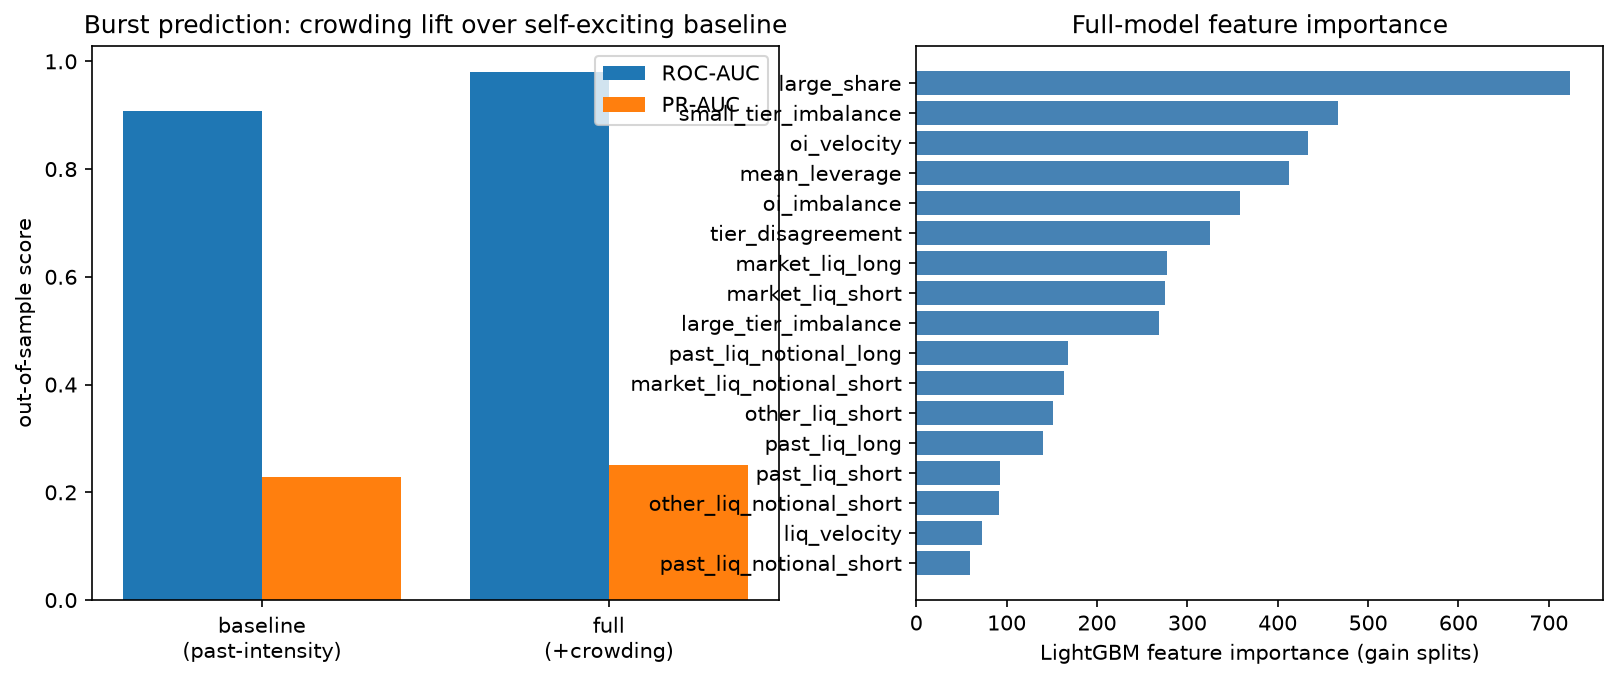
\includegraphics[width=0.92\textwidth]{../pipeline/outputs/b01_burst_baseline/burst_baseline_lift.png}
    \caption{Dự báo bùng phát trên giai đoạn kiểm tra theo thời gian, an toàn không rò rỉ. Trái: ROC-AUC và PR-AUC ngoài mẫu cho mô hình nền LightGBM tự kích thích (chỉ cường độ trễ) so với mô hình đầy đủ đã tinh chỉnh ($+$đông đúc$+$khối lượng$+$liên tài sản). Phải: mức độ quan trọng của đặc trưng (feature importance) LightGBM của mô hình đầy đủ, thể hiện đóng góp tương đối của đặc trưng đông đúc theo tầng và liên tài sản so với mô hình nền cường độ trễ. Xem Bảng~\ref{tab:m2} để so sánh đầy đủ với các mô hình nền Hawkes cổ điển và THP thần kinh.}
    \label{fig:m1}
\end{figure}

\paragraph{Báo cáo hỗ trợ.} {\sloppy Các báo cáo thử nghiệm chi tiết tại \texttt{m0-magnet-findings.md}, \texttt{m0-burst-findings.md}, \texttt{m1-crowding-lift-findings.md}, \texttt{m2-baselines-findings.md}.\par} Trích dẫn công trình liên quan (\S\ref{sec:related}--\ref{sec:gap}) được liệt kê dưới đây; các mục được đánh dấu \emph{[unverified]} trong \texttt{references.bib} đã xác nhận tiêu đề/mã arXiv nhưng cần kiểm tra tác giả/nơi công bố trước bản nộp cuối cùng.

\bibliographystyle{plainnat}
\bibliography{../references}

\end{document}
